% !TeX root = ../main.tex
% Add the above to each chapter to make compiling the PDF easier in some editors.

\chapter{Concept}\label{chapter:concept}
The following chapter presents the main aspects of a checkpoint management system (CMS), and how these functionalities could be realised. For each aspect a decision is made, resulting in a complete conceptualisation.
\section{Location}
The first issue is the location of the manager. There are two main approaches for this. One would be to have a single checkpoint manager running on every ECU, which is responsible for the checkpoints generated by the RTCR on its respective machine, and the other is one CMS component which manages the entire system. In the former approach, on ECU breakdown, another manager would then need to be selected through communication between every manager to retrieve the checkpoint and restore it on its own ECU. This star topology communication, and the fact that such a system would make more sense integrated into RTCR, makes this approach unfeasible. 
The latter, more sensible solution, would be a centralised management system which receives checkpoints from the RTCR components on their respective ECUs is proposed. This manager both stores the checkpoints and is responsible for their migration and restoration on another system. This however marks a single point of failure in the entire infrastructure, reducing system resilience and therefore rendering the manager useless. Thus redundancy is used in the form of at least two checkpoint management systems running on different ECUs and performing identical tasks. 
\section{Receiving of Checkpoints}
The next key question to be answered is how the manager gains access to the checkpoints made by RTCR. For this, three possible solutions are compared.
\subsection{Publish/Subscribe}
The first thing that comes to mind to resolve the issue of sending checkpoints on the side of the RTCR and receiving them on the side of the CMS is a simple publish and subscribe system. Here, all instances of RTCR connect to an interface set up by the manager and then send checkpoints over Ethernet whenever a new one is created. This approach is commendable for its simplicity of both concept and implementation, but has a couple of flaws: first being due to the redundancy of management systems, the manager is not transparent to the RTCR, because checkpoints have to be sent to every instance of the checkpoint manager. Another major problem is that for many RTCR components which in turn manage many components, lots of network traffic in form of checkpoints is sent to only one interface of the centralised checkpoints management system. This will quickly lead to network congestion. Therefore a solution where the CMS can receive checkpoints at its own pace is desired and presented in the following subsection.
\subsection{Distributed Shared Memory}
The DSM implemented by Weidinger, which was presented in section \ref{section:DSM} is the obvious choice for this approach. It makes it possible to exchange checkpoints between one RTCR instance and the at least two redundant instances of CMS transparently, since the RTCR theoretically never directly has to address the CMS. The missing consistency module of Weidinger's DSM doesn't present an issue here, as the RTCR would be the only component writing into the shared memory. In the possible case of CMS and an instance of RTCR operating on the same ECU, a simple shared memory utilising Genode dataspace capabilities is used. The RTCR checks for this when it attempts to establish the DSM, and in case it resides on the same ECU, the RPC interface is used.

Once the DSM is established, the CMS would then have to monitor the dataspace and store a checkpoint to their own memory whenever a change is detected. Unfortunately this kind of detection is not feasible, as the CMS itself never has direct access to the memory the RTCR writes to. Two possibilities of resolving this issue are described. Firstly, there is the naive solution of serialising and downloading all new checkpoints at set intervals. The advantage of this approach is its simplicity, but it suffers heavily from the chance of increasing checkpoint age when having to fallback farther than the granularity of the RTCR checkpointing interval. Mitigating this issue by increasing the interval entails massive network load, as a whole array of checkpoints is downloaded frequently. The second solution, a hybrid between the approaches publish/subscribe and the DSM is presented in the following section.
\subsection{Hybrid}
In this solution the receipt of checkpoints does not rely on downloading intervals. Here the RTCR broadcasts a notification whenever it writes a new checkpoint to its shared memory, containing the memory address of the updated checkpoint. The CMS can then use the IP-address from the IP-header, finds, serialises, and downloads the checkpoint in a newly spawned thread. The advantage of this approach is that it resolves all disadvantages of the naive “downloading at intervals” solution. Therefore, it would seem like the obvious choice, however one caveat exists: To maintain transparency of the redundant managers, every RTCR has to broadcast a small amount of data whenever a checkpoint is made, perhaps containing sensitive information. For many RTCRs handling many components the volume of messages might overload the network. This is only an issue for the current concept, as it would be resolved whenever the DSM functionality is integrated into is participants: due to this integration, the RTCR knows the IP-addresses of its participants, and can thus replace the broadcast with a multicast. Transparency suffers due to this hybrid solution, but overall is deemed negligible, as the addresses of the checkpoint management systems are only used for this single multicast, which can be implemented in a completely flexible fashion concerning the number of redundant checkpoint managers. Furthermore addressing the management systems is necessary in scope of migration and restoration anyway, as outlined in the eponymous section. 
\newline \newline
Altogether, the decision has to be made in favour of the hybrid solution, as it unites the positives of both the publish/subscribe and DSM approaches, with only a few drawbacks remaining.
\section{Checkpoint Storage}
After receipt of the checkpoints, the next step is to store them securely. The best way of achieving this and avoiding the vulnerability of local checkpoint storage, would be to have both management systems store them on the same network addressed storage in RAID configuration. The possibility of single point of failure is resolved due to the storage being configured in RAID, which enables both the main and the redundant system to write to the same memory. Therefore it is not necessary to integrate two network addressed storages into the infrastructure.

For purposes of efficient retrieval, the CMS and NAS have to define a primary key identifying a checkpoint uniquely. The decision for this key was made in favour of a combination of MAC-address and memory offset of the checkpoint on the machine it originated from. The MAC, offset, and serialised checkpoint will then be composited into an object containing all the necessary information. Figure \ref{fig:store_activity} depicts the control flow of storing such a checkpoint.
\begin{figure}
    \centering
    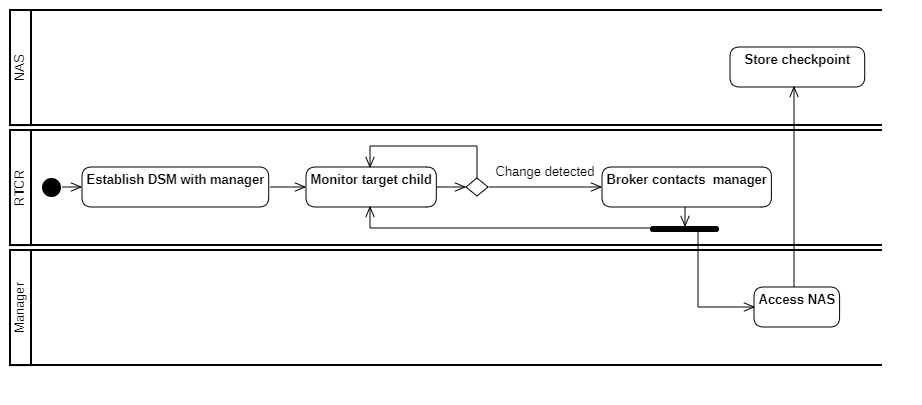
\includegraphics[width=\textwidth]{Images/checkpoint-storing_activity.png}
    \caption{Activity diagram visualising storing of checkpoints.}
    \label{fig:store_activity}
\end{figure}
\section{Migration and Restoration}\label{section:Migration_and_Restoration}
There are two different scenarios where migration and restoration is necessary. The first being when one of the RTCR components asks the CMS to migrate and restore one of its programs, for example for load balancing reasons. In this case the MAC-address and offset of the checkpoint have to be transmitted. The CMS then retrieves the serialised checkpoint from memory and selects the ECU to restore it on.

The second case is that the ECU or the RTCR thereon stops working entirely. For this purpose, it is assumed that the CMS knows of the event and the MAC-address of the board it occured on. All checkpoint objects with that MAC-address are then retrieved and restored one by one on another selected machine.
The selection for both scenarios is made by comparing the ECUs in the network using different performance metrics. These metrics are
\begin{itemize}
    \item CPU load
    \item RAM usage
    \item Capability quota
\end{itemize}
of the ECU. Since this information is not accessible over network through any already existing Genode interface, the RTCR has to provide such an interface, whereupon demand it accesses CPU load, RAM usage, and capability quota locally.

One big issue is that the redundancy of managers warrants that they have to agree upon which component performs the restoration and thereby avoid duplicate processes. As timing differences of the managers might make one ECU more or less suitable than it was at migration time of another checkpoint manager, the possibility of them restoring the checkpoint on different platforms has to be acknowledged. The decision is therefore made at the time of checkpoint retrieval. Whichever is the first to access a checkpoint from the NAS, is the one to migrate and restore the checkpoint. This is enforced by a mutex and the immediate deletion of the checkpoint from the database. This is necessary in any case, as both offset and MAC-address are those of the old host of the process and therefore expired. 

The entire process of migration and restoration is shown in figure \ref{fig:migr_activity}.
\begin{figure}
    \centering
    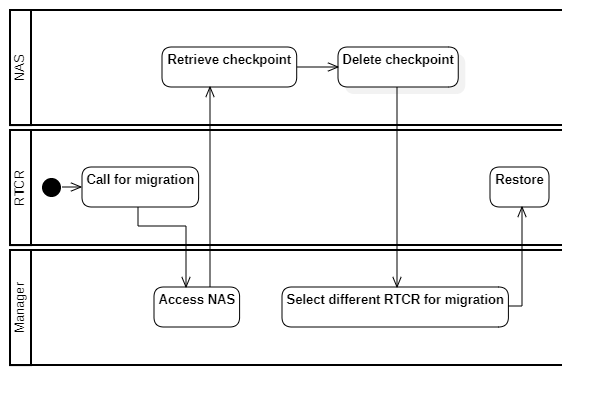
\includegraphics[width=0.75\textwidth]{Images/migration-restoration_activity.png}
    \caption{Activity diagram visualising migration and restoration.}
    \label{fig:migr_activity}
\end{figure}
\section{Considerations outside of Implementation Scope}
The following sections touch on aspects of a checkpoint management system, that are important to consider given its foundations, but were deemed too time-intensive to be within the scope of the implementation.
\subsection{Knowing a Restoration is Necessary}
For the CMS to provide failure safety while still avoiding redundant inactive ECUs, it needs to know that either the ECU itself or the RTCR component failed. The naive solution is to implement heartbeats into every single RTCR component, which are then checked by the CMS. If the heartbeat from an ECU stops, a migration and restoration is performed. This approach can be either accomplished with the RTCR multicasting a heartbeat to the managers or with the CMS requesting a heartbeat from an RTCR interface, both with a set interval. These solutions heavily utilise the network and therefore put it under unnecessary load. Fortunately, the architecture of KIA4SM provides a more sensible resolution: because of the homogeneity of ECUs and the resulting possibility of any process running on any ECU, some sort of meta-entity has to exist, which distributes the processes to their systems at the beginning, and later schedules them. Such an entity would also be responsible for notifying the manager of system failures.

\subsection{Managing Checkpoints in Real Time}
An important aspect of RTCR is its real-time capability, which warrants a discussion concerning the real-time capability of the system managing the RTCR instances, even though it is not part of the practical implementation. There are two aspects that may hinder the target child at fulfilling its schedules. One of them is the obvious loss of time of needing to migrate and restore the program, which has to be mitigated by increasing performance of migration and restoration, maybe by even using hardware-assisted solutions. The other aspect is the schedule on the machine that is being migrated to. If many programs with real-time demand are already in execution, the scheduler on the new ECU might have to enforce that our program misses a schedule. Resolving this completely would entail knowing the state of the scheduler on any ECU that is eligible for migration. However an estimate can be made using CPU load and RAM usage, which is already included in the current concept of ECU selection. Ultimately, both an interface providing information about current schedules on the side of RTCR and a complex module parsing this data and making decisions based on it are required.